%\documentclass[10pt,twocolumn,letterpaper]{article}
\documentclass[times,10pt,twocolumn]{article}
 
\usepackage{iccv}
\usepackage{times}
\usepackage{epsfig}
\usepackage{graphicx}
\usepackage{amsmath}
\usepackage{amssymb}
\usepackage{todonotes}
\usepackage[T1]{fontenc}
\usepackage[utf8]{inputenc}
\usepackage[english]{babel}

% Include other packages here, before hyperref.

% If you comment hyperref and then uncomment it, you should delete
% egpaper.aux before re-running latex.  (Or just hit 'q' on the first latex
% run, let it finish, and you should be clear).
\usepackage[pagebackref=true,breaklinks=true,letterpaper=true,colorlinks,bookmarks=false]{hyperref}

 \iccvfinalcopy % *** Uncomment this line for the final submission

\def\iccvPaperID{****} % *** Enter the ICCV Paper ID here
\def\httilde{\mbox{\tt\raisebox{-.5ex}{\symbol{126}}}}

% Pages are numbered in submission mode, and unnumbered in camera-ready
\ificcvfinal\pagestyle{empty}\fi
\begin{document}

%%%%%%%%% TITLE
\title{Incremental Large-Scale Multi-View Stereo}
\author{Andrea Romanoni \qquad Matteo Matteucci\\
Politecnico di Milano\\
Italy\\
{\tt\small \{andrea.romanoni,matteo.matteucci\}@polimi.it}
}

\maketitle
%\thispagestyle{empty}


\begin{abstract}
   
\end{abstract}

\section{Introduction}%%%%%%%%%%%%%%%%%%%%%%%%%%%%%
Reconstructing a 3D model of a scene acquired from a set of images is a long standing problem faced by the computer vision community. 
3D modeling has a wide variety of applications: cultural heritage, mapping for human and robot navigation and photogrammetric city reconstructions.
Early works focused on the reconstruction of point-wise sparse structure of the environment.
In the last decade, thanks to the advancement on optimization techniques,  the improvement of hardware resources, and the proposal of benchmark datasets \cite{seitz_et_al06,strecha2008},  dense reconstruction attracted the interests of many researchers.

Classical Multi-View Stereo methods \cite{gargallo2005bayesian,delaunoy_et_al_08} handle small objects, e.g., those proposed in the benchmark of Stretcha \etal \cite{strecha2006combined}.
The reasons are related both to the computational and memory resources needed to handle big set of images, and to the limitations of the optimization procedures.
The common volumetric voxel-based representation of the space requires a huge amount of memory to store accurate and detailed data.
Thanks to the introduction of hashing methods and especially  Delaunay Triangulation based methods, algorithms to deal with large-scales scenes have been proposed.
Successful Delaunay-based incremental approaches have been proposed in \cite{lovi_et_al_11,hoppe2013incremental,litvinov_lhuillier_13,romanoni15b,romanoni15a} but they all rely sparse data and visibility-only information, therefore the final reconstruction lacks in details and is not photo-consistent.

The remarkable work of Vu \etal \cite{vu_et_al_2012} achieves very accurate results since they directly optimize the model according to the images. 
Two limitations affect this work: the processing of the images is the batch, and the reconstruction pipeline is not fully automatic, since the optimization method is well suited for 2-manifold meshes, but the method proposed to estimate the initial mesh does not guarantee that manifold property holds for the whole model.
In this paper we propose a framework to overcome this  limitations.

To our knowledge this paper presents the first incremental algorithm for large-scale environments, which reconstruct a dense, continuous and photo-consistent manifold mesh. 
We propose a fully automatic pipeline that integrates an existing manifold reconstruction algorithm proposed in \cite{romanoni15a} with the accurate surface evolving refinement step of Vu \etal \cite{vu_et_al_2012} improved and extended to work incrementally and a novel manifold-preserving mesh merging algorithm.

Section \ref{sec:related_works} reviews related literature, in particular, about incremental reconstruction; Section \ref{sec:incremental_dense}  presents an overview of our system. 
Section \ref{sec:exp} shows the experimental results and finally Section \ref{sec:concl} concludes the paper underlining some future extensions of the presented framework.

\section{Related works}%%%%%%%%%%%%%%%%%%%%%%%%%%%%%%5
\label{sec:related_works}
Among all dense 3D reconstruction algorithm proposed in the literature, here we focus on incremental reconstruction systems. 

A very popular class of reconstruction algorithms relies on depth maps; they first estimate the depth map for a selected set of keyframe, then they merge the depth maps into a single consistent 3D model of the scene. 
An early work was presented by Pollefeys \etal in \cite{pollefeys_et_al_08}: they estimate the depth maps with the classical plane-sweeping \cite{collins1996space}, for each depth map they create a 3D rectangle mesh of two triangles that covers all the depth image, then each triangle is subdivided iteratively where discontinuity or non-planarity in the depth map region enclosed in the triangle occurs. The meshes generated for each depth maps are finally registered and the redundant triangles are deleted.
Newcombe \etal \cite{newcombe2010live} estimate keyframe depth maps by interpolating the points from Structure from Motion with radial basis function, and by  refining them the with the dense optical flow correspondences; then they merge the depth map into a single model.
DTAM \cite{newcombe2011dtam} improved the previous method by estimating depth maps with bundles of small-parallax images; it registers the points from the depth map to the estimated surface, and it updates a volumetric Truncated Signed Distance Function (TSDF) according the depth data. 
The author in \cite{stuhmer2012parallel,stuckler2014multi} proposed similar approaches, while \cite{concha2015incorporating} improved on DTAM by incorporating planar and layout priors in the estimation. 


Most of the previous depth maps-based approaches rely on a voxel-based volumetric representation of the TSDF and are not suitable for large-scale reconstruction. Sch{\"o}ps \etal \cite{schops20153d} propose then to use voxel hashing together with a careful filtering of noisy depth data.
Even if the results are very remarkable, the resulting model is a non-continuous mesh, and the meshing step is not directly driven by the images, but by marching cubes \cite{lorensen1987marching} that interpolates the TSDF , as in most of the depth map based approaches.

Mesh-based algorithm represents an effective alternative to depth-maps based reconstruction. Labatut \etal \cite{labatut2007efficient} estimate directly a visibility and photo-consistent mesh from the Delaunay triangulation of the 3D noisy points obtained from the depth maps.
Vu \etal  \cite{vu_et_al_2012} improve this algorithm by estimating an initial visibility-consistent mesh then by evolving the mesh such that it maximizes the photo-consistency with respect to the images. 
These Delaunay-based volumetric approaches are able to handle large scale scenes, but both \cite{labatut2007efficient} and \cite{vu_et_al_2012} process all the images together, therefore they are not incremental.

\section{System Overview}%%%%%%%%%%%%%%%%%%%%%%%%%%
\label{sec:incremental_dense}
We propose a novel a fully automatic and incremental pipeline that combines three steps to reconstruct a photo-consistent model of the environment: \emph{manifold reconstruction}, \emph{mesh merging} and \emph{windowed photo-metric refinement} (Figure \ref{fig:architecture}). 
The inputs of our system are the 3D points position, the camera poses and the visibility rays, estimated by any incremental SfM or SLAM algorithm such as the method implemented in openMVG or \cite{moulon2012adaptive} or ORB-SLAM \cite{mur2015orb}. 
%In Figure \ref{fig:architecture} we illustrate a scheme of the whole system. 
%Every  $W$ frames the system outputs the available reconstruction.
 
 \begin{figure}[t]
  \centering
  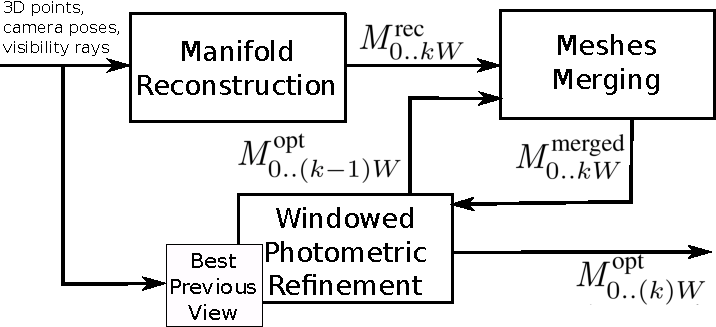
\includegraphics[width=0.48\textwidth]{pipeline}
  \caption{Architecture of the incremental reconstruction system}
  \label{fig:architecture}
\end{figure}

%\todo{TODO Visibility and}
We process these inputs every $W$ images through the manifold reconstruction algorithm proposed by Romanoni \etal \cite{romanoni15b}, which estimates incrementally a low-resolution manifold mesh from sparse data, named  $\mathit{M}_{0..kW}^{\text{rec}}$, with $k \in \mathbb{N}$. 
In the initial case of $k=1$ we directly refine the manifold mesh through the windowed photo-metric refinement, leading to a mesh named $\mathit{M}_{0..W}^{\text{opt}}$.
Instead, for $k>1$ we need to combine the low-resolution mesh $\mathit{M}_{0..kW}^{\text{rec}}$ with the previously refined mesh $\mathit{M}_{0..(k-1)W}^{\text{opt}}$. 

The windowed photo-metric refinement evolves the mesh surface in order to maximize the photo-consistency between pairs of cameras, in a similar fashion to the method proposed by Vu \etal \cite{vu_et_al_2012} which have been proved to scale well with large-scale scenes.
To keep the pipeline scalable, we compare a constant number of camera pairs instead of comparing all the possible pairs of cameras. 
Therefore, in our incremental setting, the choice of the camera pairs we would compare is crucial to enable a good trade-off between  accuracy and scalability.
We propose a novel algorithm (implemented in the \emph{best previous views} block of Figure \ref{fig:architecture}) that chooses the best camera pairs based on the mutual per-pixel mean parallax angle we compute by relying on the existing model of the scene.

We combine the high-resolution refined mesh  $\mathit{M}_{0..(k-1)W}^{\text{opt}}$  with the new low-resolution manifold $\mathit{M}_{0..kW}^{\text{rec}}$ through a novel mesh merging approach that keeps the manifold property valid and updates the topology. 
The output of this module is the multi-resolution mesh $\mathit{M}_{0..kW}^{\text{merged}}$.
After such multi-resolution merging step the refinement algorithm is able to jointly refine both the newly added region together with the refined part.


\subsection{Parallax Weighted Photometric refinement}%%%%%%%%%%%%%%%%%%%%%%%%%%%%%%%%%%%%%%%%%%%%%%%%%%%%%%%%%%%%%%%%%%%%%%%%%
\label{subsec:photo}
Once a new set of $W$ frames have been processed to possibly update the current model with a new region of the scene, we refine it photometrically. 
First, we increase the resolution of the mesh in order to represent fine-grained details, through One-to-four midpoint subdivision algorithm.
Then we apply the photo-consistent mesh evolution process.
Our approach have been inspired by the methods proposed by Pons \etal \cite{pons2007multi} and Vu \etal
\cite{vu_et_al_2012} and extended to process coherently incremental data. 
We minimize an energy:
\begin{equation}
\label{eq:en}
E = E_{\textrm{photo}} + E_{\textrm{smooth}},
\end{equation}
where  $E_{\textrm{photo}}$ represents the energy induced by  the photo-consistency of the model with respect to the images, and $E_{\textrm{smooth}}$ is a prior energy that enforces the smoothness of the surface. 

\begin{figure}[t]
\centering
  \def\svgwidth{200pt}
  \input{cameproj.pdf_tex}
\caption{Variables involved in the photometric refinement process}.
\label{fig:cameraproj}
\end{figure}

We first explain how to minimize $E_{\textrm{photo}}$.
Let consider two images $I$ and $J$, and a point $x$ belonging to the surface $\mathit{S}$ (Figure \ref{fig:cameraproj}); then, $err_{A, B}(x)$ is a function that decreases if the similarity between the patch around the projection of $x$ in  $A$ and $B$ increases, e.g., in our case, the inverse ZNCC of the $4$ pixels neighborhood.
The energy $E_{\textrm{photo}}$ in Equation \eqref{eq:en} becomes:
\begin{align}
\label{eq:energy_photo}
\begin{split}
  E_{\textrm{photo}} = E(\mathit{S}) & = \sum_{i,j}\int_{\Omega^{\textrm{S}}_{i,j}} err_{I, I_{ij}^{\mathit{S}}}(x_i)\textrm{d}x_i \\
  &= \sum_{i,j} \mathit{err}^{im}_{ij}(x),
\end{split}
\end{align}
where the term $I_{ij}^{\mathit{S}}$ represents the reprojection of the image from the $j$-th camera in the image $I$ through the surface $\mathit{S}$.
Now, let $X_i \in \mathbb{R}^3$ be a vertex of the surface mesh $\mathit{S}$ and $\phi_i(x)$ be the barycentric coordinates of a surface point $x$ in the triangle  with vertex $X_i$.
The discrete gradient of $E_{\textrm{photo}} = E(\mathit{S})$ computed for a vertex $X_i$ is:
\begin{align}
\begin{split}
  \frac{\textrm{d}E(\mathit{S})}{\textrm{d}X_i}& =  \int_{\mathit{S}} \phi_i(x) \nabla E(x) \textrm{d}x = \\
  & = \int_{\mathit{S}} \phi_i(x) \nabla (\sum_{i,j} err^{im}_{ij}(x)) \textrm{d}x\\
  & = \int_{\mathit{S}} \phi_i(x) \sum_{i,j} \nabla err^{im}_{ij}(x)\textrm{d}x.
\end{split}
\end{align}
We are now able change the variable of integration in order to integrate the energy over image $I$.
Let define $\overrightarrow{n}$ as the normal at $x$ pointing outward the surface $\mathit{S}$, $x_i$ the projection of x into the $I$ image, $\mathbf{d}_i$ as the vector from camera $i$ to $x$, $z_i$ as the depth of $x$ in camera $i$ (see Figure \ref{fig:cameraproj}). 
With the change of variable $\textrm{d}x_i = -\overrightarrow{n}^T \mathbf{d}_i \textrm{d}x/z_i^3$ \cite{pons2007multi} we obtain:
\begin{equation}
\label{eq:final}
  \frac{\textrm{d}E(\mathit{S})}{\textrm{d}X_i} = 
  \sum_{i,j} \int_{\Omega^{\textrm{S}}_{i,j}} 
  \phi_i(x)  \nabla err^{im}_{ij}(x)\frac{z_i^3}{\overrightarrow{n}^T \mathbf{d}_i }\overrightarrow{n} \textrm{d}x_i,
\end{equation}
where $\Omega_{i,j}$ represents the surface region that induces the projection of image $J$ into the image $I$.

To minimize the term $E_{\textrm{photo}}$, in the batch approach proposed in \cite{vu_et_al_2012}, the authors apply  the gradient descent optimization by moving the vertices of the mesh.
According to Equation \eqref{eq:final}, for each vertex, they collect the gradient contributions from each incident facet and from each pair of cameras viewing the vertex itself.
In our incremental case we could simply modify this process to take into account the cameras and images up to the current time and all the possible pairs. 
However this often would cause drifting in the evolution process: in a typical incremental scenario illustrate in Figure \ref{fig:increm}(a), we evolve the surface with only a subset of cameras; therefore, the gradient collected in $v$ receives contributions  only from small baseline pairs of cameras, e.g., $C_1-C_2$, $C_1-C_3$ and $C_2-C_3$, which induce high uncertainty in the estimation.
Instead, in the batch case of Figure \ref{fig:increm}(b), wide baseline and  small baseline pairs symmetric to $C_1$, $C_2$ and $C_3$ pairs contributions are able to nicely mitigate this effect.


Since we are dealing with incremental data, in general, we cannot predict where new images are going to be captured, however we propose to mitigate the issue described thus far, by including a parallax weight in the gradient contributions that favors good baseline against small or too wide pairs.
We turn Equation \eqref{eq:final} into:
\begin{equation}
\label{eq:my_final}
  \frac{\textrm{d}E(\mathit{S})}{\textrm{d}X_i} = 
  \sum_{i,j} \int_{\Omega^{\textrm{S}}_{i,j}} 
  \phi_i(x)  \mu(x) \nabla err^{im}_{ij}(x)\frac{z_i^3}{\overrightarrow{n}^T \mathbf{d}_i }\overrightarrow{n} \textrm{d}x_i,
\end{equation}
where we compute the weight $\mu(x)$ from the angle $\theta$ between the viewing rays of the current pair of cameras incident in $x$ as:
\begin{equation}
\label{eq:weight}
\mu(x) = e^{-\frac{(\frac{\pi}{2}-\theta)^2}{2*\frac{\pi}{4}^2}}.
\end{equation}
Equation \eqref{eq:weight}  represents the value of an un-normalized Gaussian centered in $\frac{\pi}{2}$ and standard deviation $\frac{\pi}{4}$, indeed the more the parallax is close to $\frac{\pi}{2}$ the more accurate the estimation. 
We rely on this guideline also to choose the best pairs of cameras to use in the evolution process (Section \ref{subsec:pair}).



The evolution process is complemented with the umbrella operator \cite{wardetzky2007discrete}, which moves each vertex in the mean position of its neighbors that approximates the Laplace-Beltrami operator to minimize the energy $E_{\textrm{smooth}}$.


\begin{figure}[t]
\centering
\setlength{\tabcolsep}{1px}
\begin{tabular}{cc}
  {\def\svgwidth{0.23\textwidth}
  \input{increm02.pdf_tex}}&
  {\def\svgwidth{0.23\textwidth}
  \input{increm01.pdf_tex}}\\
  (a)&(b)
\end{tabular}
\caption{Camera contribution in the (a) incremental  and (b) batch cases}
\label{fig:increm}
\end{figure}

% The discrete vector field $v$ associates to each $i$-th vertex a vector $v_i$ defined such that $v(x) = \sum_i \phi_i(x) v_i$.

\begin{figure*}[t]
\centering
\setlength{\tabcolsep}{1px}
\begin{tabular}{ccc}
{\def\svgwidth{0.32\textwidth}
  \input{meshmerge01.pdf_tex}}&
{\def\svgwidth{0.32\textwidth}
  \input{meshmerge02.pdf_tex}}&
{\def\svgwidth{0.32\textwidth}
  \input{meshmerge03.pdf_tex}}\\
(a)&(b)&(c)\\
{\def\svgwidth{0.32\textwidth}
  \input{meshmerge04.pdf_tex}}&
{\def\svgwidth{0.32\textwidth}
  \input{meshmerge05.pdf_tex}}&
{\def\svgwidth{0.32\textwidth}
  \input{meshmerge06.pdf_tex}}\\
(d)&(e)&(f)\\
\end{tabular}
\label{fig:mesh_merging}
\caption{Mesh merging steps}
\end{figure*}


\subsubsection{Model-based best Pairs}
\label{subsec:pair}
At each iteration of our incremental algorithm process, we process a new set of $W$ images, and we need to define which camera pairs we compare in the evolution algorithm.
The naive solution compares each new camera with all the new and the old $N$ ones.
This approach has two drawbacks: first the complexity grows linearly with the number of cameras ($\mathbb{O}((W+N)*W) = \mathbb{O}(N)$); second, we include in the evolution process too narrow or too distant cameras which lead to noisy gradient due to their unfavorable parallax.

We overcome the first drawback by limiting the number of camera compared for each new camera to $N_{\text{comp}}=3$ pairs, such that the complexity is constant.
The second drawback requires an analysis of the camera mutual parallax, \ie, the angle of the viewing rays that look the same 3D point.
We propose to exploit the current 3D model of the scene to compute the average parallax $P$ among two cameras with centers $c_{\text{ref}}$ and $c_i$:
\begin{equation}
 P = \frac{1}{A_{\mathit{S}}}  \int_{\mathit{S}} \phi_i \phi_j atan2(cos(\angle(\overrightarrow{c_{\text{ref}}x})),sin(\angle(c_{i}x))) \textrm{d}x
\end{equation}
where $A_{\mathit{S}}$ is the area of the visible mesh surface $\mathit{S}$, and $x$ is a point on $\mathit{S}$.

Given this computation for all possible pair very efficiently performed on GPU, for each new camera $c_{\text{ref}}$  we choose the best $N_{\text{comp}}=3$  which induce the average parallax closer to $\frac{\pi}{2}rad$.




\begin{figure*}[t]
\centering
\setlength{\tabcolsep}{1px}
\begin{tabular}{cccc}
{\def\svgwidth{0.23\textwidth}
  \input{whymanifold03.pdf_tex}}&
{\def\svgwidth{0.23\textwidth}
  \input{whymanifold04.pdf_tex}}&
{\def\svgwidth{0.23\textwidth}
  \input{whymanifold01.pdf_tex}}&
{\def\svgwidth{0.23\textwidth}
  \input{whymanifold02.pdf_tex}}\\
(a)&(b)&(d)&(e)\\
\end{tabular}
\label{fig:whymanifold}
\caption{}
\end{figure*}

\subsection{Manifold-Preserving Mesh Merging}
\label{sub:merge}
One of the key steps of our incremental pipeline to work fully automatic is the manifold-preserving mesh merging which aims at jointly merging two meshes with different resolutions, and keeping the manifold property valid.

We propose an approach different from existing methods such as \cite{turk1994zippered} and \cite{VuPhD011} which deal with meshes with similar resolution and significant overlap.
Indeed, in our case, we need to merge two meshes with  different resolutions, \ie, the refined and the rough meshes, such that, when they overlap, we  keep the refined part and reject the rough one; moreover,  since the refined mesh could evolve significantly far from the low resolution one, the meshes sometimes does not have a good overlap.



The idea of our mesh merging is to estimate narrow corresponding path that become boundaries of the two meshes; then connect the endings of these paths and treat such polygonal line as a hole of the joint mesh and fill it with a manifold-preserving hole filling algorithm.




Let $\mathit{M}$ and  $\mathit{M}^{\text{opt}}$ be the new manifold and the refined mesh, \eg, blue and green meshes in Figure \ref{fig:mesh_merging}(a). 
We build the bounding boxes around the facets of the two meshes, and we detect which box from the refined mesh intersect a box from the new mesh and we remove the corresponding facets, as the red facets in Figure \ref{fig:mesh_merging}(b).
Since the bounding boxes circumscribe the facets from low resolution mesh $\mathit{M}$, they self-adapt to cope with not good overlapping region.
Indeed, big facets, and then big boxes, correspond to regions of the mesh estimated from few 3d points, therefore the uncertainty is high; on the other side, small facets and small bounding boxes correspond to denser 3D points and consequently less uncertain regions of the mesh $\mathit{M}$, where $\mathit{M}$ is likely to be close to $\mathit{M}^{\text{opt}}$.


Once we removed the facets from intersecting boxes, $\mathit{M}$ splits into a set of connected submeshes; we select the biggest submesh, named  $\mathit{{M}_{big}}$.
We order the edges of boundary of $\mathit{{M}_{big}}$ into a list $\mathit{b} = \{b_1, \dots,  b_n\}$.
Let $T_{\text{init}}$ be the number of the triangle of  $\mathit{M}$; if the triangles of $\mathit{{M}_{big}}$ are lower than a threshold $\tau_{bm}=30\% (T_{\text{init}})$, it means that the overlapping with the refined mesh is predominant and we stop the merging process, keeping the refined mesh as output.

If the process continues, we retrieve the set of bounding boxes around the facets adjacent to the border $\mathit{b}$, \ie, the gray facets in Figure \ref{fig:mesh_merging}(d), and we find the set $\mathit{F}^{\text{opt}}$ of facets  belonging to the refined mesh which intersects these bounding boxes, \eg, the green facets  in Figure \ref{fig:mesh_merging}(d).
The boundary edges of $\mathit{F}^{\text{opt}}$ populate the list  $\mathit{b}^{\text{opt}} = \{b_1^{\text{opt}}, \dots,  b_m^{\text{opt}}\}$, and, among these edges, we select the vertices  $v_{\text{start}}^{\text{opt}}$ and $v_{\text{end}}^{\text{opt}}$ which are the vertices nearest to the extremity $v_{\text{start}}$ and  $v_{\text{end}}$ of the boundary $\mathit{b}$ (see Figure \ref{fig:mesh_merging}(e)). 
We estimate the path  $\mathit{b}^{\text{fin}}$ from $v_{\text{start}}^{\text{opt}}$ to $v_{\text{end}}^{\text{opt}}$ among the edges of the facets  $\mathit{F}^{opt}$ such that it minimizes the energy:
\begin{equation}
  E_{\text{path}} = \sum_i E(b_i^{\text{opt}})= \sum_i \angle (\overrightarrow{n}_i^{\text{opt}},\overrightarrow{n}_i^{\text{new}})
\end{equation}
where $\overrightarrow{n}_i^{\text{opt}}$ is the normal of the facet among $\mathit{F}^{opt}$ adjacent to  $b_i^{\text{opt}}$; and
$\overrightarrow{n}_i^{\text{new}}$ is the normal of the facet defined by the two extremities $A$ and $B$ of edge ${b}^{\text{opt}}$ and the nearest vertex $C \in \mathit{b}$.
We minimize $E_{\text{path}}$ with the Dijkstra algorithm  and we extract the final boundary $\mathit{b}^{\text{fin}} = \{ b_1^{\text{fin}}, \dots, b_s^{\text{fin}}\}$ (Figure \ref{fig:mesh_merging}(e)).

Finally, we connect $v_{\text{start}}^{\text{opt}}$ to $v_{\text{start}}$  and $v_{\text{end}}^{\text{opt}}$ to  $v_{\text{end}}$ such that we create a closed polyline $\{v_{\text{start}}^{\text{opt}},  v_{\text{start}}, \mathit{b}, v_{\text{end}}^{\text{opt}}, v_{\text{end}}, \mathit{b}^{\text{fin}}\}$, that we fill with the manifold-preserving algorithm proposed in \cite{liepa2003filling}  (Figure \ref{fig:mesh_merging}(f)). 
To handle the possible topology change of the mesh, we iterate this process for all the boundaries of the mesh  $\mathit{\bar{M}}_{0..kW}$, not negligible, \ie, smaller than $\tau_{\text{top}}= 15\%$ the biggest boundary.

The final mesh $\mathit{M}^{\text{merged}}$ is composed by all the facets from the refined mesh $\mathit{M}^{\text{opt}}$ which have not been removed by the previous process, the submeshes kept from the new mesh $\mathit{M}$ and finally the facets created to fill the polylines.


\subsection{Why manifold}
Both the reconstruction algorithm from sparse data we adopt in our pipeline and the merging in Section \ref{sub:merge} focus the attention on preserving the manifold property of the mesh.
Let recall that the manifold property holds if and only if each vertex $v$ of the surface mesh is \emph{regular}, \ie, if and only if the edges opposite to $v$ form a closed path without loops  \cite{litvinov_lhuillier_13}.

The sources of non-manifoldness can be induced by tetrahedra intersecting at a vertex, and by tetrahedra with a common edge (non-manifold edge). 
In both cases the non-manifoldness can be fixed, in principle, by cloning and offsetting the vertex of intersection, but two big drawbacks arise: this process applied to the 3D triangulation would invalidate the Delaunay property; and, since many non-manifold vertices are generated, rearranging the triangulation and the visibility information for each non-manifold point becomes inefficient. For these two reasons we directly prevent the generation of non-manifold configurations.
%%resolution

The surface evolution method described in Section \ref{subsec:photo}, collects the contributions of the gradient from the images, for each vertex of the mesh \eqref{eq:final}.
Therefore non-manifold meshes, would collect non-consistent contributions leading to misleading evolution. 
For instance in Figure \ref{fig:whymanifold}(a), Equation \eqref{eq:final} for the vertex $v$ sums up the gradient contribution carried by the triangles $T_1$, $T_2$, $T_3$ and $T_4$ (Figure \ref{fig:whymanifold}(b)); since the corresponding normals have very different directions, these contributions and the resulting vector flows contain contradictory information.
On the other side, Figure \ref{fig:whymanifold}(c) shows a similar shape, but the mesh is manifold and the gradients collected in $v_1$ and $v_2$ (Figure \ref{fig:whymanifold}(d)) lead to a coherent mesh evolution.





\section{Experimental Results}
\label{sec:exp}

\section{Conclusions and Future works}
\label{sec:concl}

\subsection{Paper length}
eight pages in length. One additional page containing cited references is allowed,

{\small
\bibliographystyle{ieee}
\bibliography{biblioTotal}
}

\end{document}
